\documentclass{standalone}
\usepackage{tikz}
\begin{document}
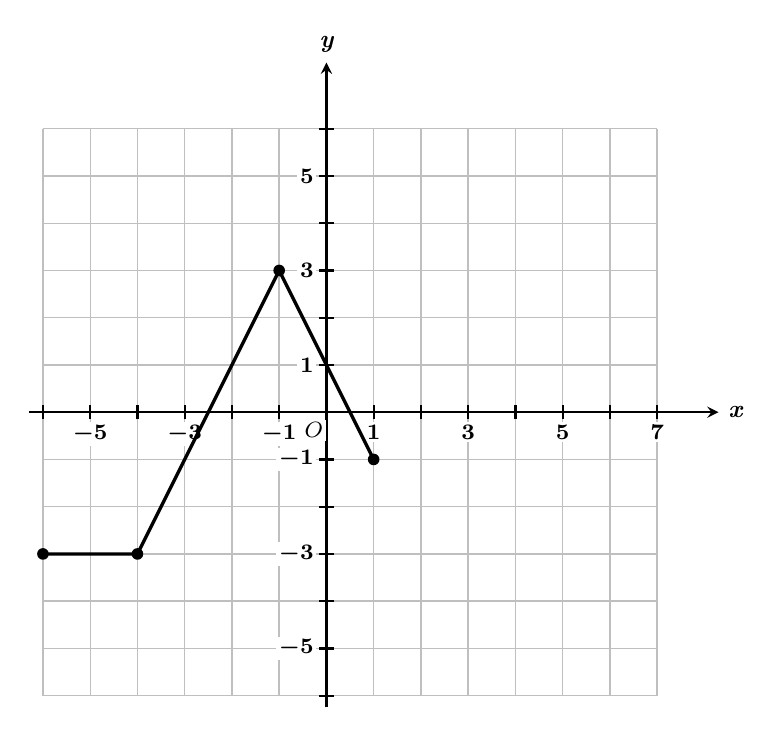
\begin{tikzpicture}[color=black, >=stealth, scale=0.6]
  % Grid: x from -6 to 7, y from -6 to 6
  \draw[gray!50, line width=0.5pt] (-6,-6) grid (7,6);
  % Axes
  \draw[->, thick] (-6.3,0) -- (8.3,0);
  \draw[->, thick] (0,-6.25) -- (0,7.4);
  \node[font=\small\bfseries\itshape, anchor=west] at (8.3,0) {x};
  \node[font=\small\bfseries\itshape, anchor=south] at (0,7.4) {y};
  % Tick marks at every integer
  \foreach \x in {-6,...,7} \draw[thick] (\x,-0.15) -- (\x,0.15);
  \foreach \y in {-6,...,6} \draw[thick] (-0.15,\y) -- (0.15,\y);
  % Tick labels at odd values only
  \foreach \x in {-5,-3,-1,1,3,5,7}
    \node[font=\footnotesize\boldmath, fill=white, inner sep=1pt, anchor=north] at (\x,-0.2) {$\x$};
  \foreach \y in {-5,-3,-1,1,3,5}
    \node[font=\footnotesize\boldmath, fill=white, inner sep=1pt, anchor=east] at (-0.2,\y) {$\y$};
  \node[font=\footnotesize, fill=white, inner sep=1pt, anchor=north east] at (0,-0.15) {$O$};
  % Piecewise-linear graph with filled endpoints/vertices
  \draw[line width=1.2pt] (-6,-3) -- (-4,-3) -- (-1,3) -- (1,-1);
  \foreach \p in {(-6,-3),(-4,-3),(-1,3),(1,-1)}
    \fill[black] \p circle (3.5pt);
\end{tikzpicture}
\end{document}
